\documentclass{beamer}

\usepackage{graphicx}
\usepackage{framed}

\begin{document}

%=====================================================================%
\begin{frame}
\frametitle{McNemar Test}
\Large
\textbf{McNemar Test}
\begin{itemize}
\item McNemar's test is a statistical test used on paired nominal data. 
\item It is applied to $2 \times 2$ contingency tables with a dichotomous trait, with matched pairs of subjects, to 
determine whether the row and column marginal frequencies are equal (that is, whether there is "marginal homogeneity").
\end{itemize}

\end{frame}
%=====================================================================%
\begin{frame}
\frametitle{McNemar Test}
\Large

\begin{itemize}
\item Binary Outcomes (Success and Failure)
\item Before and After 
\item Is there is a significant difference between "Before" and "After" is terms of success rates

\end{itemize}


\end{frame}
%=====================================================================%
\begin{frame}
\frametitle{McNemar Test}
\Large
\begin{itemize}
\item The test is applied to a $2 \times 2$ contingency table, which tabulates the outcomes of two tests on a sample of n subjects, as follows.

\end{itemize}
\begin{figure}
\centering
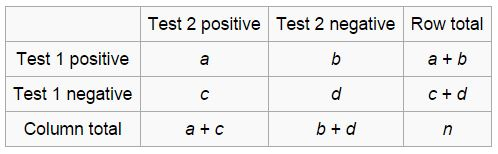
\includegraphics[width=0.99\linewidth]{./mcmenar1}
%\caption{}
%\label{fig:mcmenar2}
\end{figure}



\end{frame}
%=====================================================================%
\begin{frame}
\frametitle{McNemar Test}
\Large
\begin{itemize}
\item The null hypothesis of marginal homogeneity states that the two marginal probabilities for each outcome are the same, i.e. \[p_a + p_b = p_a + p_c\] and \[p_c + p_d = p_b + p_d.\]
\item Thus the null and alternative hypotheses are
\end{itemize}
\begin{align}
H_0 & :~p_b=p_c \\
H_1 & :~p_b \ne p_c
\end{align}


\end{frame}
%=====================================================================%
\begin{frame}
\frametitle{McNemar Test}
\Large
\begin{itemize}
%\item Here $p_a$, etc., denote the theoretical probability of occurrences in cells with the corresponding label.
\item The McNemar test statistic is:
\[\chi^2 = {(b-c)^2 \over b+c}.\]

\end{itemize}




\end{frame}
%=====================================================================%
\begin{frame}[fragile]
\frametitle{McNemar Test}
\Large
\texttt{mcnemar.test() }
\begin{itemize}
\item Agresti (1990), p. 350.
\item Presidential Approval Ratings.
\item Approval of the President's performance in office in two surveys,
one month apart, for a random sample of 1600 voting-age Americans.
\end{itemize}

\end{frame}
%=====================================================================%
\begin{frame}
\frametitle{McNemar Test}
\Large
\begin{itemize}
\item In the first example, a researcher attempts to determine if a drug has an effect on a particular disease. 
\item Counts of individuals are given in the table, with the diagnosis (disease: present or absent) before treatment given in the rows, and the diagnosis after treatment in the columns. 
\item The test requires the same subjects to be included in the before-and-after measurements (matched pairs).
\end{itemize}


\end{frame}
%=====================================================================%
\begin{frame}
\frametitle{McNemar Test}
\Large
\begin{figure}
\centering
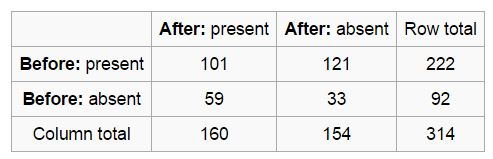
\includegraphics[width=0.99\linewidth]{./mcmenar2}
%\caption{}
%\label{fig:mcmenar2}
\end{figure}


\end{frame}
%=====================================================================%
\begin{frame}
\frametitle{McNemar Test}
\Large
\begin{itemize}
\item In this example, the null hypothesis of "marginal homogeneity" would mean there was no effect of the treatment. 
\item From the above data, the McNemar test statistic:
\[\chi^2 = {(121 - 59)^2 \over {121 + 59}}\]
has the value 21.35, which is extremely unlikely to form the distribution implied by the null hypothesis ($P < 0.001$). 
\item Thus the test provides strong evidence to reject the null hypothesis of no treatment effect.
\end{itemize}



\end{frame}
%=====================================================================%
\begin{frame}[fragile]
\large
\texttt{mcnemar.test() }
\begin{framed}
\begin{verbatim}
Effect <-
matrix(c(101,121,59,33),
       nrow = 2,
       dimnames = list(
        "Before" = c("Present", "Absent"),
        "After" = c("Present", "Absent")))

\end{verbatim}
\end{framed}

\end{frame}
%=====================================================================%
\end{document}